\subsection{Applications of Integrals}
\subsubsection{Area Between Curves}
We have seen how to find the area between a curve and the axis but what about the area between curves? To do this, we define a new function to be the difference between the two curves. $h(x)=f(x)-g(x)$\\
$$A=\int_b^a(f(x)-g(x))dx,\text{ for }f(x)>g(x)$$
It is important that $f(x)>g(x)$ is order to obtain a positive area. We must also pay attention to cases where the functions interlace. When this happens, we will need to split it into multiple integrals to obtain positive values.\\
Ex: Area bounded by $f(x)=x+2$ and $g(x)=x^2-4$\\
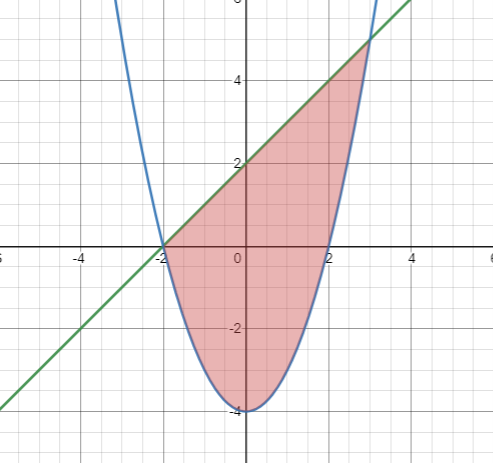
\includegraphics[scale=0.5]{Images/IntegralCalcPictures/AreaBetweenCurvesEx1.png}
\begin{align*}
    &\text{Intercepts:}\\
    &x+2=x^2-4\\
    &x^2-x-6=0\\
    &(x-3)(x+2)=0\\
    &x=3,\,x=-2\\
    &\text{check }f(x)>g(x)\text{ for }x\in(-2,3)\\
    &A=\int_{-2}^3((x+2)-(x^2-4))dx=\int_{-2}^3(-x^2+x+6)dx=\brsquare{-\frac{x^3}{3}+\frac{x^2}{2}+6x}_{-2}^3\\
    &=\frac{125}{6}
\end{align*}
Ex2: Area bounded by $y=x^3-x$ and $y=3x$\\
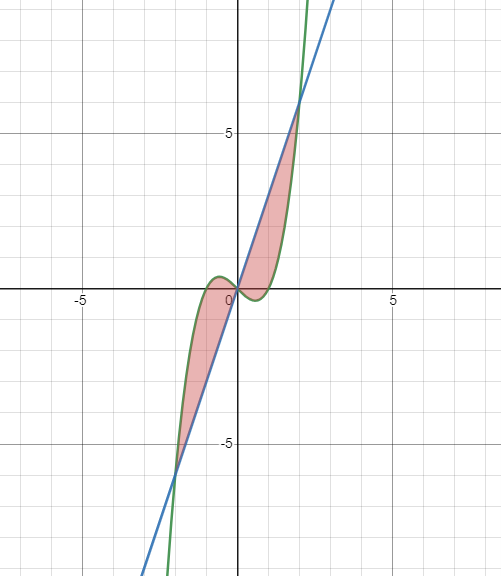
\includegraphics[scale=0.5]{Images/IntegralCalcPictures/AreaBetweenCurvesEx2.png}
\begin{align*}
    &\text{Intercepts:}\\
    &x^3-x=3x\\
    &x^3-4x=0\\
    &x(x^2-4)=0\\
    &x=0,\,x=\pm2\\
    &x^3-x>3x\text{ for }x\in(-2,0)\\
    &3x>x^3-x\text{ for }x\in(0,2)\\
    &A=\int_{-2}^0((x^3-x)-3x)dx+\int_0^2(3x-(x^3-x))dx\\
    &A=\brsquare{\frac{x^4}{4}-2x^2}_{-2}^0+\brsquare{-\frac{x^4}{4}+2x^2}_0^2\\
    &=8
\end{align*}
Alternatively, you could have recognized this as an odd function and found the area of one sector and multiplied it by 2.\\
Sometimes it may prove easier to integrate with respect to $y$ instead of $x$.\\
Ex3: Area bounded by $y^2=4x$ and $4x-3y=4$\\
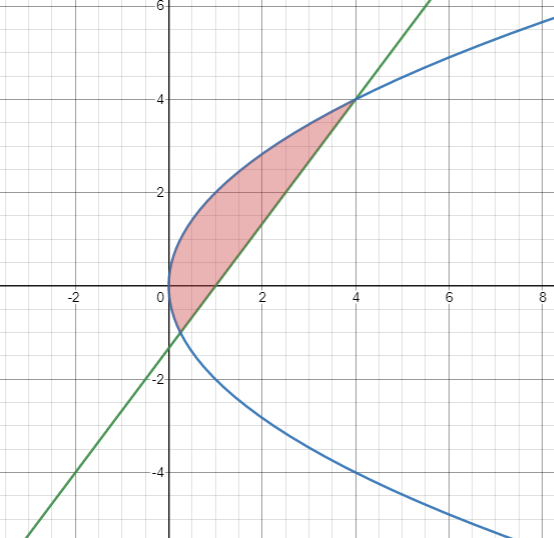
\includegraphics[scale=0.5]{Images/IntegralCalcPictures/AreaBetweenCurvesEx3.png}
\begin{align*}
    &x=\frac{y^2}{4},\,x=\frac{3}{4}y+1\\
    &y^2=4+3y\Ra y^2-3y-4=0\\
    &(y-4)(y+1)=0\Ra y=4,\,y=-1\\
    &\frac{3}{4}y+1>\frac{y^2}{4}\text{ for }y\in(-1,4)\\
    &A=\int_{-1}^4\brround{\brround{\frac{3}{4}y+1}-\frac{y^2}{4}}dy=\brsquare{\frac{3y^2}{8}+y-\frac{y^3}{12}}_{-1}^4\\
    &=\frac{125}{24}
\end{align*}
\subsubsection{Volumes of Revolution}
Consider a function $y=f(x)$. By rotating the function about the x-axis, we can create a 3D solid of revolution.\\
Disk Method:\\
If we split our function into many different rectangles of width $\Delta x$, when we revolve our function about the x-axis, we get many disks of radius $f(x_i^*)$ and width $\Delta x$. So the volume of each disk will be $V_i=\pi (f(x_i^*))^2\Delta x$. Summing these together, we get
$$V=\lim_{n\to \infty}\sum_{i=1}^n\pi(f(x_i^*))^2\Delta x=\pi\int_a^b(f(x))^2dx$$
Ex: Find the volume of the cone formed by rotating $y=\frac{x}{2}$ about the x-axis on the interval $[0,6]$
\begin{align*}
    V=\pi\int_0^6\brround{\frac{x}{2}}^2dx=\frac{\pi}{4}\int_0^6x^2dx={\frac{\pi x^3}{12}}\eval_0^6=18\pi
\end{align*}
Ex2: Find the volume of the sphere formed by rotating $y=\sqrt{r^2-x^2}$ about the x-axis
\begin{align*}
    V&=\pi\int_{-r}^r(r^2-x^2)dx=\pi\brsquare{r^2x-\frac{x^3}{3}}_{-r}^r\\
    &=\frac{4}{3}\pi r^3
\end{align*}
If we are dealing with multiple sections we can compute the volumes independently and subtract the inner volume from the outer volume
$$V=V_{outer}-V_{inner}$$
Ex3: Find the volume of the bowl formed by rotating the area bounded by $\sqrt{3-3x}$ and $\sqrt{1-x^2}$ between $x=0$ and $x=1$
\begin{align*}
    &\sqrt{3-3x}>\sqrt{1-x^2}\text{ for }x\in[0,1)\\
    &\text{Outer: }\sqrt{3-3x}\\
    &\text{Inner: }\sqrt{1-x^2}\\
    &V=\pi\int_0^1\brround{(3-3x)-(1-x^2)}dx=\pi\brsquare{2x-\frac{3}{2}x^2+\frac{x^3}{3}}_0^1\\
    &=\frac{5\pi}{6}
\end{align*}
Using the disk method, if you rotate about the x-axis, you must integrate with respect to $x$. If you rotate about the y-axis, you must integrate with respect to $y$.\\
If you are rotating about any axis other than the x or y-axis, (such as the line $y=3$, you must translate all functions so that you are rotating about the x or y-axis.\\
Ex4: Find the volume of the solid generated by rotating the region bounded by $y=0$, $x=4$, and $y=\sqrt{x}$ about the line $x=6$
\begin{align*}
    &\text{Integrate with respect to $y$: }y=\sqrt{x}\Ra x=y^2\\
    &\text{Outer: }x=y^2\\
    &\text{Inner: }x=4\\
    &\text{Bounds: }x=0\Ra y=0,\,x=4\Ra y=2\\
    &V=\pi\int_{y=0}^{y=2}\brround{(y^2)^2-(4)^2}dy\\
    &\text{Shift: }x\to x-6\\
    &V=\pi\int_0^2\brround{(y^2-6)^2-(-2)^2}dy\\
    &V=\pi\brsquare{\frac{y^5}{5}-4y^3+32y}_0^2\\
    &=\frac{192}{5}\pi
\end{align*}
Shell Method:\\
An alternative way to find area is using shells. This involves finding the are of each shell of the solid like the layers of an onion.\\
The general expression is
$$V=\int_a^b2\pi rhdr$$\\
Depending on your variable of integration, $r$ and $h$ will take the values of $x$ or $y$\\
Ex5: Using the same example as before: Find the volume of the solid generated by rotating the region bounded by $y=0$, $x=4$, and $y=\sqrt{x}$ about the line $x=6$
\begin{align*}
    &h=\sqrt{x}\\
    &r=6-x\\
    &V=2\pi\int_0^4(6-x)\sqrt{x}dx\\
    &V=2\pi\brsquare{4x^{3/2}+\frac{2}{5}x^{5/2}}_0^4\\
    &=\frac{192}{5}\pi
\end{align*}

\subsubsection{Arc Length}
Calculus is founded on the basis that any line is straight if we zoom in enough. This interpretation is very helpful when computing the length of a curve\\
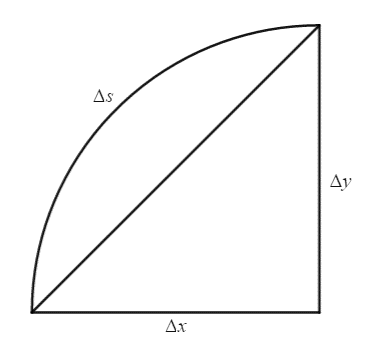
\includegraphics[scale=0.7]{Images/IntegralCalcPictures/ArcLengthTriangle.png}
\begin{align*}
    &(\Delta s)^2\approx (\Delta x)^2+(\Delta y)^2\\
    &\to(ds)^2=(dx)^2+(dy)^2\\
    &ds=\sqrt{(dx)^2+(dy)^2}\\
    &ds=\sqrt{(dx)^2+(dy)^2}\brround{\frac{dx}{dx}}\\
    &ds=\sqrt{1+\brround{\frac{dy}{dx}}^2}dx\\
    &s=\int_b^a\sqrt{1+(f'(x))^2}dx
\end{align*}
where $s$ is the arc length.\\
Ex: Find the arc length of a semicircle or radius 1
\begin{align*}
    &y=\sqrt{1-x^2}\\
    &y'=\frac{-x}{\sqrt{1-x^2}}\\
    &ds=\sqrt{1+\frac{x^2}{1-x^2}}=\sqrt{\frac{1}{1-x^2}}\\
    &s=\int_{-1}^1\frac{dx}{\sqrt{1-x^2}}={\arcsin x}\eval_{-1}^1\\
    &=\pi
    \end{align*}
Ex2: Find the length of the parabola $y=x^2$ from 0 to $a$
\begin{align*}
    &y=x^2\Ra y'=2x\\
    &ds=\sqrt{1+4x^2}dx\\
    &s=\int_0^a\sqrt{1+4x^2}dx\\
    &\vdots\\
    &=\brsquare{\frac{1}{4}\ln|2x+\sqrt{1+4x^2}|+\frac{1}{2}x\sqrt{1+4x^2}}_0^a
\end{align*}
\subsubsection{Surface Area}
We can compute some surface areas using rotations and by calculating the surface of rotation.\\
Similar to volumes of revolution, we can compute the surface area using rings: ${dS=\text{circumference}\cdot ds}$\\
$\Ra dS=2\pi y ds$\\
Ex: Find the surface area of a sphere of radius $r$
\begin{align*}
    &y=\sqrt{r^2-x^2}\\
    &y'=\frac{-x}{r^2-x^2}\\
    &ds=\sqrt{1+\frac{x^2}{r^2-x^2}}dx=\sqrt{\frac{r^2}{r^2-x^2}}dx\\
    &S=\int_{-r}^r2\pi\sqrt{r^2-x^2}\sqrt{\frac{r^2}{r^2-x^2}}dx=2\pi\int_{-r}^r rdx\\
    &S={2\pi rx}\eval_{-r}^r\\
    &=4\pi r^2
\end{align*}
Ex2: Find the surface area of a torus (doughnut). Let $R$ be the distance from the hole to the center of the solid and let $r$ be the internal radius.
\begin{align*}
    &(x-R)^2+y^2=r^2\\
    &y=\sqrt{r^2-(x-R)^2}\\
    &y'=\frac{-(x-R)}{r^2-(x-R)^2}\\
    &ds=\sqrt{1+\frac{(x-R)^2}{r^2-(x-R)^2}}dx=\frac{r}{\sqrt{r^2-(x-R)^2}}dx\\
    &dS=\frac{2\pi rx}{\sqrt{r^2-(x-R)^2}}dx\Ra S=2\pi r\int_{R-r}^{R+r}\frac{x}{\sqrt{r^2-(x-R)^2}}\\
    &u=x-R\Ra x=u+R\Ra du=dx\\
    &S=2\pi r\int_{-r}^r\frac{u+R}{\sqrt{r^2-u^2}}du=2\pi r\brround{\int_{-r}^r\frac{u}{\sqrt{r^2-u^2}}+R\int_{-r}^r\frac{du}{\sqrt{r^2-u^2}}}\\
    &\text{note that }\int_{-r}^r\frac{u}{\sqrt{r^2-u^2}}\text{is odd so it will be 0}\\
    &\Ra S=4\pi rR\int_{0}^r\frac{du}{\sqrt{r^2-u^2}}=4\pi rR{\arcsin\brround{\frac{u}{r}}}\eval_0^r\\
    &=4\pi^2rR
\end{align*}

\subsubsection{Work}
Work is defined to be $W=F\cdot x$\\
Ex: How much work is required to bring a book of 1kg to a height of 2m?
\begin{align*}
    &F=mg=9.81\\
    &W=F\cdot x=(9.81)(2)=19.62J
\end{align*}
If the force is not constant then we can break the action into small parts and sum them up: $dW=dF\cdot dx$. This gives a definition of work to be
$$W=\int_a^bF(x)dx$$
Ex2: A string has a length of 30cm (unstretched). A force of 20N is required to keep it stretched at a length of 40cm. How much work is required to stretch it from 30cm to 35cm? Note $F=kx$
\begin{align*}
    &\text{find $k$: }F(x)=kx,\,x=0.4-0.3=0.1m\\
    &F(0.1)=20=0.1k\Ra k=200N/m\\
    &W=\int_0^{0.05}F(x)dx=\int_0^{0.05}200xdx={100x^2}\eval_0^{0.05}\\
    &=0.25J
\end{align*}

\subsubsection{Average Value}
The average of a set of $n$ discrete values is defined as
$$\overline{x}=\frac{\sum\limits_{i=1}^nx_i}{n}$$
For a continuous function, the average is defined as
$$\overline{f(x)}=\frac{1}{b-a}\int_a^bf(x)dx$$
This formula is derived from the Mean Value Theorem:
\begin{align*}
    &\text{For }f(x)=F'(x),\\
    &f(c)=\frac{F(b)-F(a)}{b-a}\\
    &\int_a^bf(x)dx=F(b)-F(a)\\
    &\therefore\,f(c)=\frac{1}{b-a}\int_a^bf(x)dx=\overline{f(x)}
\end{align*}
Ex: Find the average height of the point on a semicircle.
\begin{align*}
    &\overline{y}=\frac{1}{r-(-r)}\int_{-r}^r\sqrt{r^2-x^2}dx\\
    &\text{let }x=r\sin\theta\Ra dx=r\cos\theta d\theta\\
    &\sqrt{r^2-x^2}=r\cos\theta\\
    &\theta=\arcsin\brround{\frac{x}{r}}\\
    &\frac{1}{2r}\int_{x=-r}^{x=r}r^2\cos\theta d\theta=\frac{r}{2}\int_{x=-r}^{x=r}\frac{1+\cos2\theta}{2}d\theta=\frac{r}{4}\brsquare{\theta+\frac{1}{2}\sin2\theta}_{x=-r}^{x=r}=\frac{r}{4}\brsquare{\theta+\frac{1}{2}\sin\theta\cos\theta}_{x=-r}^{x=r}\\
    &\overline{y}=\frac{r}{4}\brsquare{\arcsin\brround{\frac{x}{r}}+\frac{1}{2}\brround{\frac{\sqrt{r^2-x^2}}{r}}\brround{\frac{x}{r}}}_{-r}^r\\
    &=\frac{\pi r}{4}
\end{align*}
A common application is time averages. This is the average value of a periodic function over one period, denoted by $\brangle{f(x)}$. By inspection, the time average of $\sin x$ or $\cos x$ is 0, however, we can take the root mean squared average (RMS) instead to get a non-zero value.\\
Ex2: Compute the RMS average of $\cos x$: $\sqrt{\brangle{\cos^2x}}$
\begin{align*}
    &\brangle{\cos^2x}=\frac{1}{\pi}\int_0^\pi\cos^2xdx=\frac{1}{2\pi}\int_0^\pi(1+\cos2x)=\frac{1}{2\pi}\brsquare{x+\frac{1}{2}\sin x\cos x}_0^\pi\\
    &=\frac{1}{2}\\
    &\Ra\sqrt{\brangle{\cos^2x}}=\frac{1}{\sqrt{2}}
\end{align*}
Ex3: Average speed: Let $v(t)$ be the speed of a particle over $t_0\leq t\leq t_1$. What is the average speed of $t$?
\begin{align*}
    &\overline{v}=\frac{1}{t_1-t_0}\int_{t_0}^{t_1}v(t)dt={\frac{1}{t_1-t_0}x(t)}\eval_{t_0}^{t_1}=\frac{x(t_1)-x(t_0)}{t_1-t_0}=\frac{\Delta x}{\Delta t}
\end{align*}
Ex4: Find all positive values of $b$ such that the average of $f(x)=10-x^2$ on the interval $0\leq x\leq b$ is equal to 1.
\begin{align*}
    &1=\frac{1}{b-0}\int_0^b(10-x^2)dx=\frac{1}{b}\brsquare{10x-\frac{x^3}{3}}_0^b=10-\frac{b^3}{3}\\
    &\frac{b^2}{3}=9\Ra b^2=27\Ra b=\pm\sqrt{27}\\
    &b=\sqrt{27}
\end{align*}
\subsubsection{Weighted Averages}
Sometimes when taking an average, we may want to value certain points more and take a weighted average instead. A common example is when considering an object's center of mass.\\
Considering the simple case of discreet masses on a lever. The center of mass will be the location in which to place a fulcrum so that the torque on both sides of the lever is balanced. $\tau_{cw}=\tau_{ccw}$ where $\tau=F\times d=mgd$ where $d$ is the distance from the fulcrum. For discrete masses, we can express this as
$$\overline{x}=\frac{\ds\sum_{i=1}^Nm_ix_i}{\ds\sum_{i=1}^Nm_i}$$
Ex: If we have a 2kg weight at $x=1$ and a 1kg weight at $x=5$, what is the center of mass?
\begin{align*}
    \overline{x}\frac{(2)(1)+(1)(5)}{2+1}=\frac{7}{3}
\end{align*}
For continuous mass distributions, we can express the mass as the sum of a function of density:
$$\overline{x}=\frac{\ds\int_a^bx\mu(x)dx}{\ds\int_a^b\mu(x)dx}$$
Ex: A metal rod is 50cm long. Its density is given by $\mu(x)=\dfrac{1}{100-x}$ for $0\leq x\leq 50$
\begin{align*}
    \overline{x}&=\frac{\ds\int_0^{50}\frac{x}{100-x}dx}{\ds\int_0^{50}\frac{dx}{100-x}}=\frac{\ds\int_0^{50}\frac{x}{100-x}dx}{\ds\int_0^{50}\brround{\frac{x-100}{100-x}+\frac{100}{100-x}}dx}\\
    &=\frac{\ds{-\ln|100-x|}\eval_0^{50}}{\ds{\brround{-x-100\ln|100-x|}}\eval_0^{50}}\\
    &=\frac{-50+100\ln 2}{\ln 2}=100-\frac{50}{\ln 2}\approx 28.06cm
\end{align*}
The more general expression of a weighted average is
$$\overline{f(x)}=\frac{\displaystyle{\int_a^bf(x)w(x)dx}}{\displaystyle{\int_a^bw(x)dx}}$$
where $w(x)$ is the weighting applied.\\
Notice in the example of center of mass, $f(x)=x$ and $w(x)=\mu(x)$\\
Ex2: Let $R$ be the region bounded above the x-axis by $y=x$ and $y=x^3$. What is the average x-coordinate of $R$?
\begin{align*}
    &\text{Want average of $f(x)=x$ over $R$}\\
    &f(x)=x,\,w(x)=x-x^3\\
    &\mathrm{Avg}=\frac{\ds\int_0^1x(x-x^3)dx}{\ds\int_0^1(x-x^3)dx}=\frac{2/15}{1/4}=\frac{8}{15}
\end{align*}
\\
Probability:\\
We use the method of weighted averages to calculate probabilities as well.\\
Ex: Pick a point at random in $0<y<1-x^2$ (the area under the parabola). What is the probability that $x>\frac{1}{2}$?
\begin{align*}
    &P\brround{x>\frac{1}{2}}=\frac{\displaystyle{\int_{\frac{1}{2}}^1(1-x^2)dx}}{\displaystyle{\int_{-1}^1(1-x^2)dx}}\\
    &P=\frac{\ds\brsquare{x-\frac{x^3}{3}}_{\frac{1}{2}}^1}{\ds\brsquare{x-\frac{x^3}{3}}_{-1}^1}=\frac{15}{96}
\end{align*}